% Scribe template is a combination of 16831 and 10725. Thanks to those TAs!
\documentclass[11pt]{article}
\usepackage{latexsym}
\usepackage{amsmath}
\usepackage{amssymb}
\usepackage{amsthm}
\usepackage{bm}
\usepackage{epsfig}
\usepackage[tight]{subfigure}
\usepackage{hyperref}
\usepackage{listings}


\newcommand{\handout}[5]{
  \noindent
  \begin{center}
  \framebox{
    \vbox{
      \hbox to 5.78in { {#1} \hfill #2 }
      \vspace{4mm}
      \hbox to 5.78in { {\Large \hfill #5  \hfill} }
      \vspace{2mm}
      \hbox to 5.78in { {\em #3 \hfill #4} }
    }
  }
  \end{center}
  \vspace*{4mm}
}

\newcommand{\lecture}[5]{\handout{#1}{#2}{#3}{#4}{#5}}

\newtheorem{theorem}{Theorem}
\newtheorem{corollary}[theorem]{Corollary}
\newtheorem{lemma}[theorem]{Lemma}
\newtheorem{observation}[theorem]{Observation}
\newtheorem{proposition}[theorem]{Proposition}
\newtheorem{definition}[theorem]{Definition}
\newtheorem{claim}[theorem]{Claim}
\newtheorem{fact}[theorem]{Fact}
\newtheorem{assumption}[theorem]{Assumption}

% 1-inch margins, from fullpage.sty by H.Partl, Version 2, Dec. 15, 1988.
\topmargin 0pt
\advance \topmargin by -\headheight
\advance \topmargin by -\headsep
\textheight 8.9in
\oddsidemargin 0pt
\evensidemargin \oddsidemargin
\marginparwidth 0.5in
\textwidth 6.5in

\parindent 0in
%\parskip 1.5ex
\renewcommand{\baselinestretch}{1.1}

\begin{document}
\newcommand{\defeq}[0]{\ensuremath{\stackrel{\triangle}{=}}}
\def\x{\mathbf{x}}
\def\w{\mathbf{w}}
\def\K{\mathbf{K}}
\lecture{{\bf 16-822}: Geometry-based Methods in Vision (F17) }{Released: Oct-21., Due: Nov 11th}{Lecturer: Martial Hebert}{TA: Dinesh Reddy, Nate chodosh, Martin li}{Homework 3}

\section{Theory(65)}
\subsection{Affine cameras (30 Points)}
In class, we have mostly focused on perspective cameras. For this part of the homework, we consider cameras with center lying on the plane at infinity, especially {\it affine cameras}. An affine camera is one that has a camera matrix of the form $M=\left[A \,|\, b\right]$ in which A is singular and the last row of M is of the form $(0, 0, 0, 1)$. The following questions explore affine cameras a little more in depth.
\begin{itemize}
\item Given a set of points $X_i$ in $3D$, and their projection $x_i$ in the image, what is the projection of the centroid of $X_i$'s? (no equations, just 1 short line.)
\item Show that an affine camera maps parallel world lines to parallel image lines; i.e., when using an affine camera, parallel lines in $3D$ project to parallel lines in image plane.\footnote{Actually, the converse is also true; if the camera preserves parallelism of lines, then it is an affine cameras.}
\item Show that for parallel lines mapped by an affine camera, the ratio of lengths on line segments is an invariant.
\end{itemize}
For the following questions, consider a system of $2$ affine cameras, with camera matrix $M$ and $M'$: (Last row of each camera matrix is of the form $(0, 0, 0, 1)$.)
\begin{itemize}
\item Show that epipolar planes (and lines) are parallel.
\item Show that the affine fundamental matrix $F$ defined by two affine cameras is invariant to an affine transformation of the world coordinates.
\end{itemize}


\subsection{Two camera geometry (20 Points)}
Consider a pair of cameras of fundamental matrix $F$. We are interested in
the set $\mathcal{V}$ of points that project to the same point in both images. In other
words, we are interested in the set of point $P$ such that $MP = p = p' = M'P$
(but we know only $F$, not $M$ and $M'$). This is an interesting set of points
because, in a stereo system, there is no disparity at those points, so that the
images are locally the same at those points (called the ``horopter''). The matching will be the most
accurate at the points of $\mathcal{V}$.
\begin{enumerate}
\item Show that the points $p$ projection of points $P$ in $\mathcal{V}$ satisfy $p^TFp = 0$.
\ashow{$p'^TFp  = p^TFp =0$}
\item Show that any fundamental matrix $F$ can always be decomposed into
the sum of a symmetric matrix $S$ ($S = S^T$ ) and a skew-symmetric $X$
($X = -X^T$). (i.e., of the form $F = S + X$)
\ashow{$F = .5 (F + F^T) + .5 ( F - F^T)$}
\item Show that the locus of points such that $p^TFp = 0$ is a conic with
matrix $S$, using the identity $F = S + X$ (you will not need to get part 2 correct in order to answer this).
\ashow{$p^T(S + X)p = 0 \rightarrow p^TSp + p^TXp = 0 \rightarrow p^TSp = 0$  because Xp is orthogonal to p}
%\item Show that both epipoles belong to this conic.
%\ashow{$e^TFe = 0$ because $Fe=0$, thus $e^TSe =0$. Also $e'^TF^Te'=0 \dots$}
\end{enumerate}


%\subsection{Extra Credits - $\Pi$ $\|$ to the baseline (10 Points) }
%Consider a plane $\Pi$ viewed in a two-camera system. Show that if the vanishing line of $\Pi$ in one image (i.e., the projection of the line at infinity of $\Pi$ in the image) contains the epipole in that image, then $\Pi$ is parallel to the baseline between the 2 cameras (the line joining the 2 camera centers).



\subsection{Fundamental matrices between three cameras (25 Points)}
In this problem we consider the relationship between $3$ images. Let us denote by $F_{ij}$ the fundamental matrix between image $i$ and $j$ (from 1 to 3), and by $e_{ij}$ the epipole generated by image $j$ in image $i$. We will now show that the $3$ fundamental matrices induced by $3$ cameras are not independent. 

\begin{itemize}
\item Draw the 3 cameras with $e_{ij}$ labelled.
\item Show that: $F_{ij}e_{ik} = e_{jk} \times e_{ji}$ for all triplets. (this can be shown purely geometrically, without 
involved algebra)
\item Based on these 3 quadratic relations, give a counting argument showing that the 3-camera geometry is characterized by 18 degrees of freedom. And thus conclude that the $3$ fundamental matrices are not independent.
\end{itemize}

%\section{Auto-calibration (20 + 10 + 10)}
%\subsection{General Questions (20 Points)}
%\begin{enumerate}
%\item No equations, use a counting argument only: Suppose that we have
%$m$ images from which we have generated a projective reconstruction.
%Suppose that the intrinsic parameters ($K_i$) are fixed throughout all of
%the images but unknown except for the skew which is known to be $0$.
%How many images are needed to solve for the calibration parameters
%(auto-calibration toward metric reconstruction)?
%\item Can it be solved in a linear fashion in this case?
%\item Suppose that all the calibration parameters in $K$ are allowed to vary
%across the images, but that we know that the two coordinates of the
%principal point are equal in each of the images: $x_o = y_o$. How many
%images are needed to solve the auto-calibration problem?\footnote{FYI, this particular constraint does not correspond to a realistic physical constraint on the cameras, but it is still %a valid constraint in theory.}
%\item Can it be solved linearly?
%\item Linear approaches to the auto-calibration problem solve for $L = Q_3Q^T_3$,
%where $Q_3$ is the $4 \times 3$ matrix of the first three columns of the $4 \times 4$
%rectifying matrix $Q$. After solving for $L$, how can we recover $Q_3$?
%\end{enumerate}


\section{Having fun by learning from implementing! (35 Points)}
In this part of the homework, we will explore 3D reconstruction. Especially, we will study a full pipeline of a typical 3D reconstruction system using Structure from Motion (SfM) and Stereo Matching. Slight different from the previous homeworks, this time you do not implement everything from scratch. Instead, you will delve into one of the existing packages for this purpose (Here we use the {\em SFMedu} system from the computer vision group at Princeton University). You can use other state-of-the art SFM pipelines as well like \href{https://github.com/mapillary/OpenSfM}{OpenSFM}(in python) and \href{https://colmap.github.io/}{COLMAP}(in C++)) for the assignment by analyzing the results and modifying some steps of particular interest and importance. For you, this is also a very good way to understand the material taught in the class (I can say this from first hand experience). You can use any opensource SFM and MVS system for this homework. 

\subsection{What you are supposed to do:}
You need to both implement and answer questions as follows:

\begin{figure}[h!]
\centering
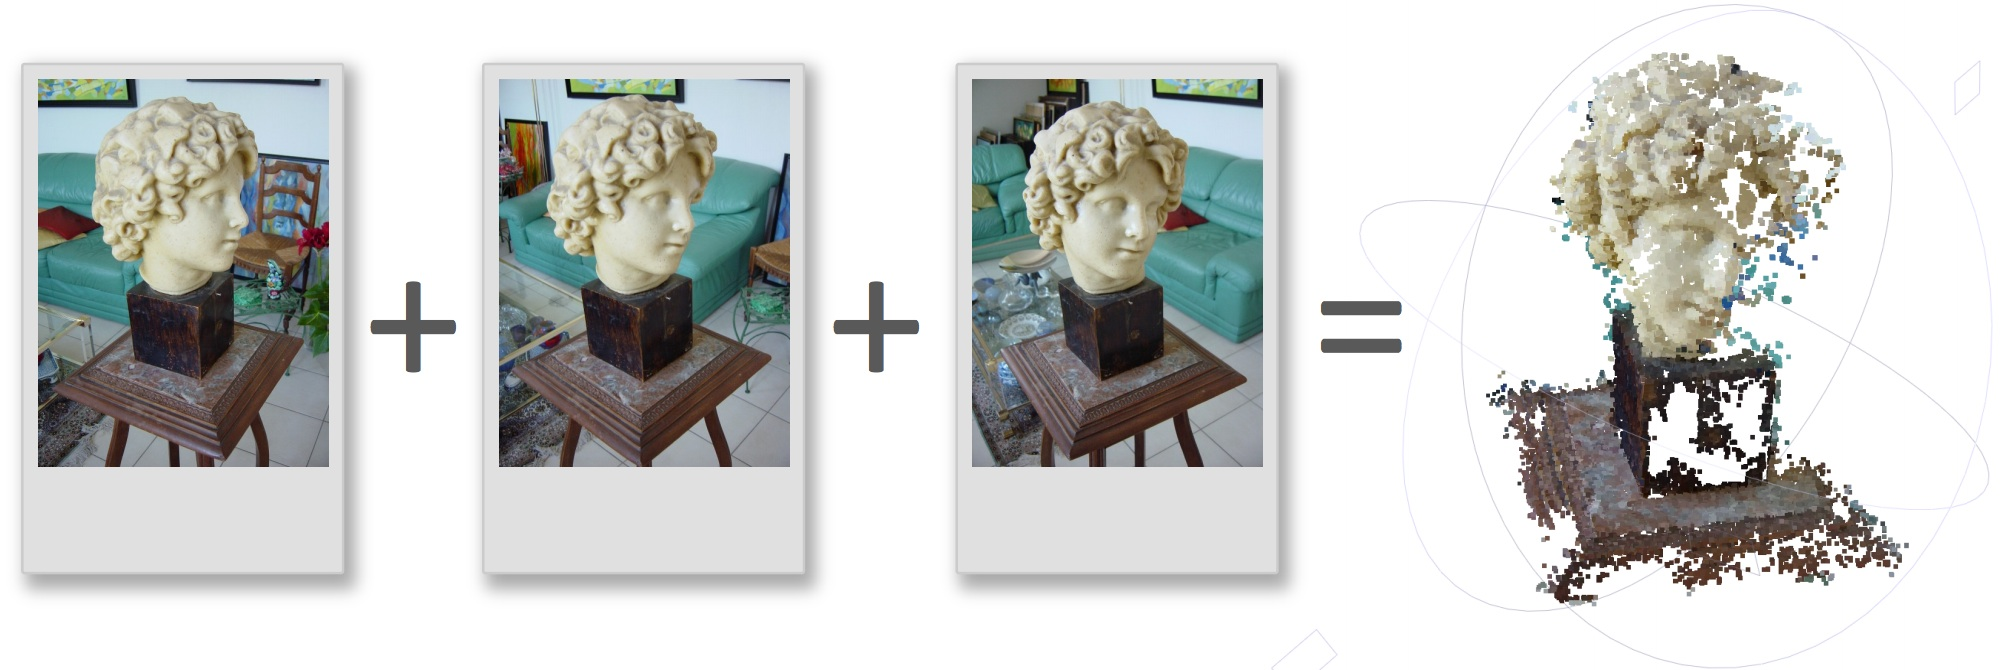
\includegraphics[width=0.9\textwidth]{tmpimages/teaser.jpg}
\caption{An illustration of the SFM system: Structure from Motion (SfM) and Stereo Reconstruction.}
\label{fig:sfmedu}
\end{figure}

\begin{itemize}
\item{{\bf{Run the SFMedu(or similar) system}}\\
I have already included the SFMedu package in $\texttt{./code/}$ folder. Run the SFMedu system by running the $\texttt{SFMedu2.m}$ script in MATLAB. Make sure that it runs successfully and produces a $\texttt{dense.ply}$ point cloud file. Install MeshLab from \url{http://meshlab.sourceforge.net}, and open the point cloud in MeshLab and rotate around the model. Take a screen capture of the point cloud and put it in the report as the answer to this question. An illustration is shown in Figure~\ref{fig:sfmedu}.}

\item{{\bf{List the Major Steps}}\\
Read the code carefully, especially $\texttt{SFMedu2.m}$. Summarize the major steps for SfM and dense stereo matching, and write it down in the report as answer to this questions.}

\item{{\bf{Principal Point}}\\
What is the assumption for the principal points in this system? Under what condition will this assumption get violated?}

\item{{\bf{Data Structure}}\\
Graph is a data structure used in the code for bundle adjustment. It has $5$ major fields. What are their names? What is the data in each field? How is the data organized? Why we need these $5$ fields?}

\item{{\bf{Reconstruct Your Own Images}}\\
Capture/Find two sequences of images (at least $5$ images per set) on some interesting objects or scenes, run the system on these images. If it fails, figure out why it fails, and change the code or retake good images until it works. Submit the input images, as well as three screen captures of your reconstruction per image set in the report. Explain all the changes or things you have to do to make it work. Which step do you think is the most unstable one? Explain why. List suggestion for a normal user without any computer vision background about how to take good images to make it work.}

\item{{\bf{Compute the Reprojection Errors}}\\
Write a function\vspace{-0.05in}
$$\texttt{function printReprojectionError(graph)}\vspace{-0.05in}$$
that takes a graph (as defined in the SFMedu system), and prints out the current reprojection error, so that you can insert the function into many steps for debugging purpose, to check if the reconstruction errors are getting smaller. A call to this function is at Line 160 of $\texttt{SFMedu2.m}$. Submit the function as code. Also, plot the reprojection errors in the report for the image sequence provided and the two sets of images you captured in the report PDF file.}

\item{{\bf{Visualize the Reprojection Points}}\\
Write a function \vspace{-0.05in}
$$\texttt{function visualizeReprojection(graph,frames)}\vspace{-0.05in}$$
that takes a graph (as defined in the SFMedu system), and draw the 3D keypoint point cloud projected onto each image, as well as their observed location. Figure~\ref{fig:visual} shows an example of the output for your function. You are required to write a function to produce the same kind of visualization. Each observed keypoint is represented by a red $\times$, and the reprojection of its 3D estimated location is represented by a green $+$, and these two points are connected by a blue line. For the 3D points that are projected to the image but not observed from the image, it should be shown as a yellow $\circ$. A call to this function is at Line 162 of $\texttt{SFMedu2.m}$. Submit the function as code, and also include the visualization results of the image sequence provided and the two sets of images you captured in the report PDF file.}

\begin{figure}[h!]
\centering
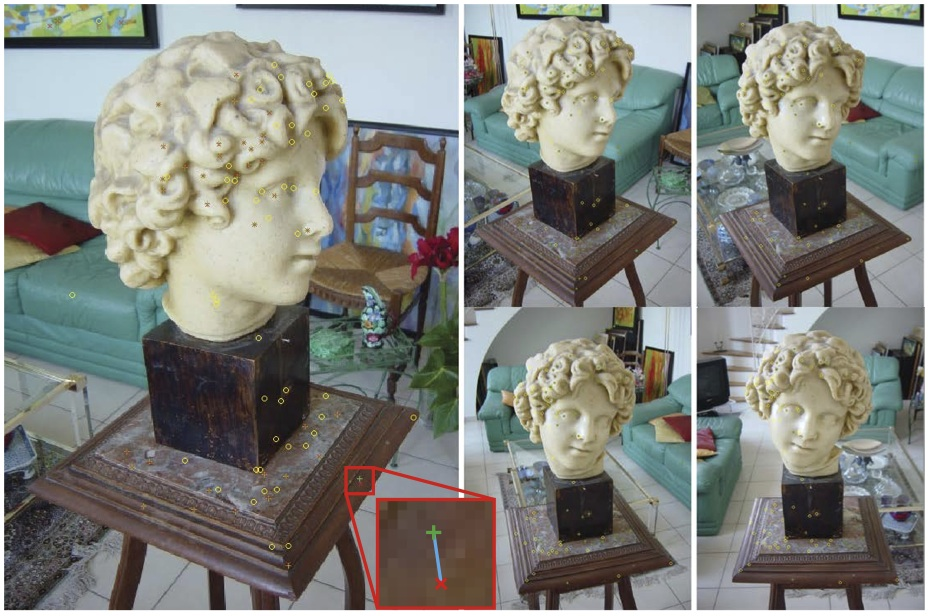
\includegraphics[width=0.95\textwidth]{tmpimages/visual.jpg}
\caption{An example result produced by \texttt{function visualizeReprojection(graph,frames)}.}
\label{fig:visual}
\end{figure}

\item{{\bf{Levenberg-Marquardt}}\\
$\texttt{bundleAdjustment.m}$ uses matlab function $\texttt{lsqnonlin}$ to minimize the objective function via the Levenberg-Marquardt algorithm: \vspace{-0.05in}
\begin{align*}
&\texttt{[vec,resnorm,residuals,exitflag] =}\\
&\texttt{lsqnonlin(@(x) reprojectionResidual(graph.ObsIdx,graph.ObsVal,px,py,f,x),}\\
&\texttt{[Mot(:);Str(:)], [], [], options);}
\end{align*}

Please read all the code and figure out what is the objective function it is optimizing for. Write down the math equation of this objective function in your report.

%The Matlab implementation lsqnonlin of Levenberg-Marquardt is not suitable for very large scale problem. Read the document of lsqnonlin and explain why this statement is true in your report.}


%\item{{\bf{Intrinsics}}\\
%Change the code to optimize for the full intrinsics matrix. Submit the code and illustrate your results.}
\end{itemize}


\subsection{What you have to submit:}
\label{sec:tosubmit}
You should submit three files:
\begin{itemize}
\item A report that contains all the images (both the images you captured and your result images) and answers to the questions.
\item Your CODE folder that contains all source code (including YOUR readme) for your system, and your ``SFMedu2.m'' script that takes no parameter as input and runs directly in Matlab to generate
the results reported in your PDF file.
\item Your IMAGE folder that contains all the input, intermediate and output images.
\end{itemize}


\subsection{Tips:}
\label{sec:helpercode}
\begin{itemize}
\item Make sure to keep ``sanity checks'' in your code while you are debugging, by checking an equation that you know should be true. (e.g., $l^TCm=0$). Keep such code commented when you submit, so that I can see and appreciate it!
\item Normalize coordinates of points before doing anything. This is important!
\item Remember the transformations that you are estimating are up to a scale.
\item Keep in mind all the things Martial mentioned in class!
\item Start early...
\item Have fun!!
\end{itemize}




\end{document}
